\documentclass{article}
\usepackage{ctex}
\usepackage{graphics}
\usepackage{geometry}
\usepackage{listings}
\usepackage[colorlinks,linkcolor=red,anchorcolor=blue,citecolor=green]{hyperref}
\setlength{\parindent}{2pt}
% bmeps -c test.png test.eps
\geometry{left=2.0cm,right=2.0cm,top=2.0cm,bottom=2.0cm}
\definecolor{cGray}{RGB}{230,230,250}
\newcommand{\code}[1]{\colorbox[RGB]{255,182,193}{\textcolor[RGB]{220,20,60}{#1}}}
\title{单变量线性回归}
\author{pwlin1992@gmail.com}
\begin{document}
\maketitle
\tableofcontents
\begin{large}
  \section{模型表示}
  \paragraph{例子}\mbox{} \\
  \indent 根据房子的大小,给出房子的价格。

  这是一个监督学习,因为对于每个训练数据,我们都知道其房子大小所对应的价格。更具体一点,这是回归问题,因为最终的结果是一个连续变量。

  \begin{enumerate}
  \item m

    训练集中实例的数量
  \item x

    特征/输入变量
  \item y

    目标变量/输出变量
  \item (x, y)

    训练集中的实例
  \item $(x^{(i)}, y^{(i)})$

    第i个观察实例
  \item h

    学习算法的解决方案或函数,也称为假设
  \end{enumerate}

  \paragraph{监督学习算法的工作方式}\mbox{} \\
  \begin{figure}[h]
    \centering
    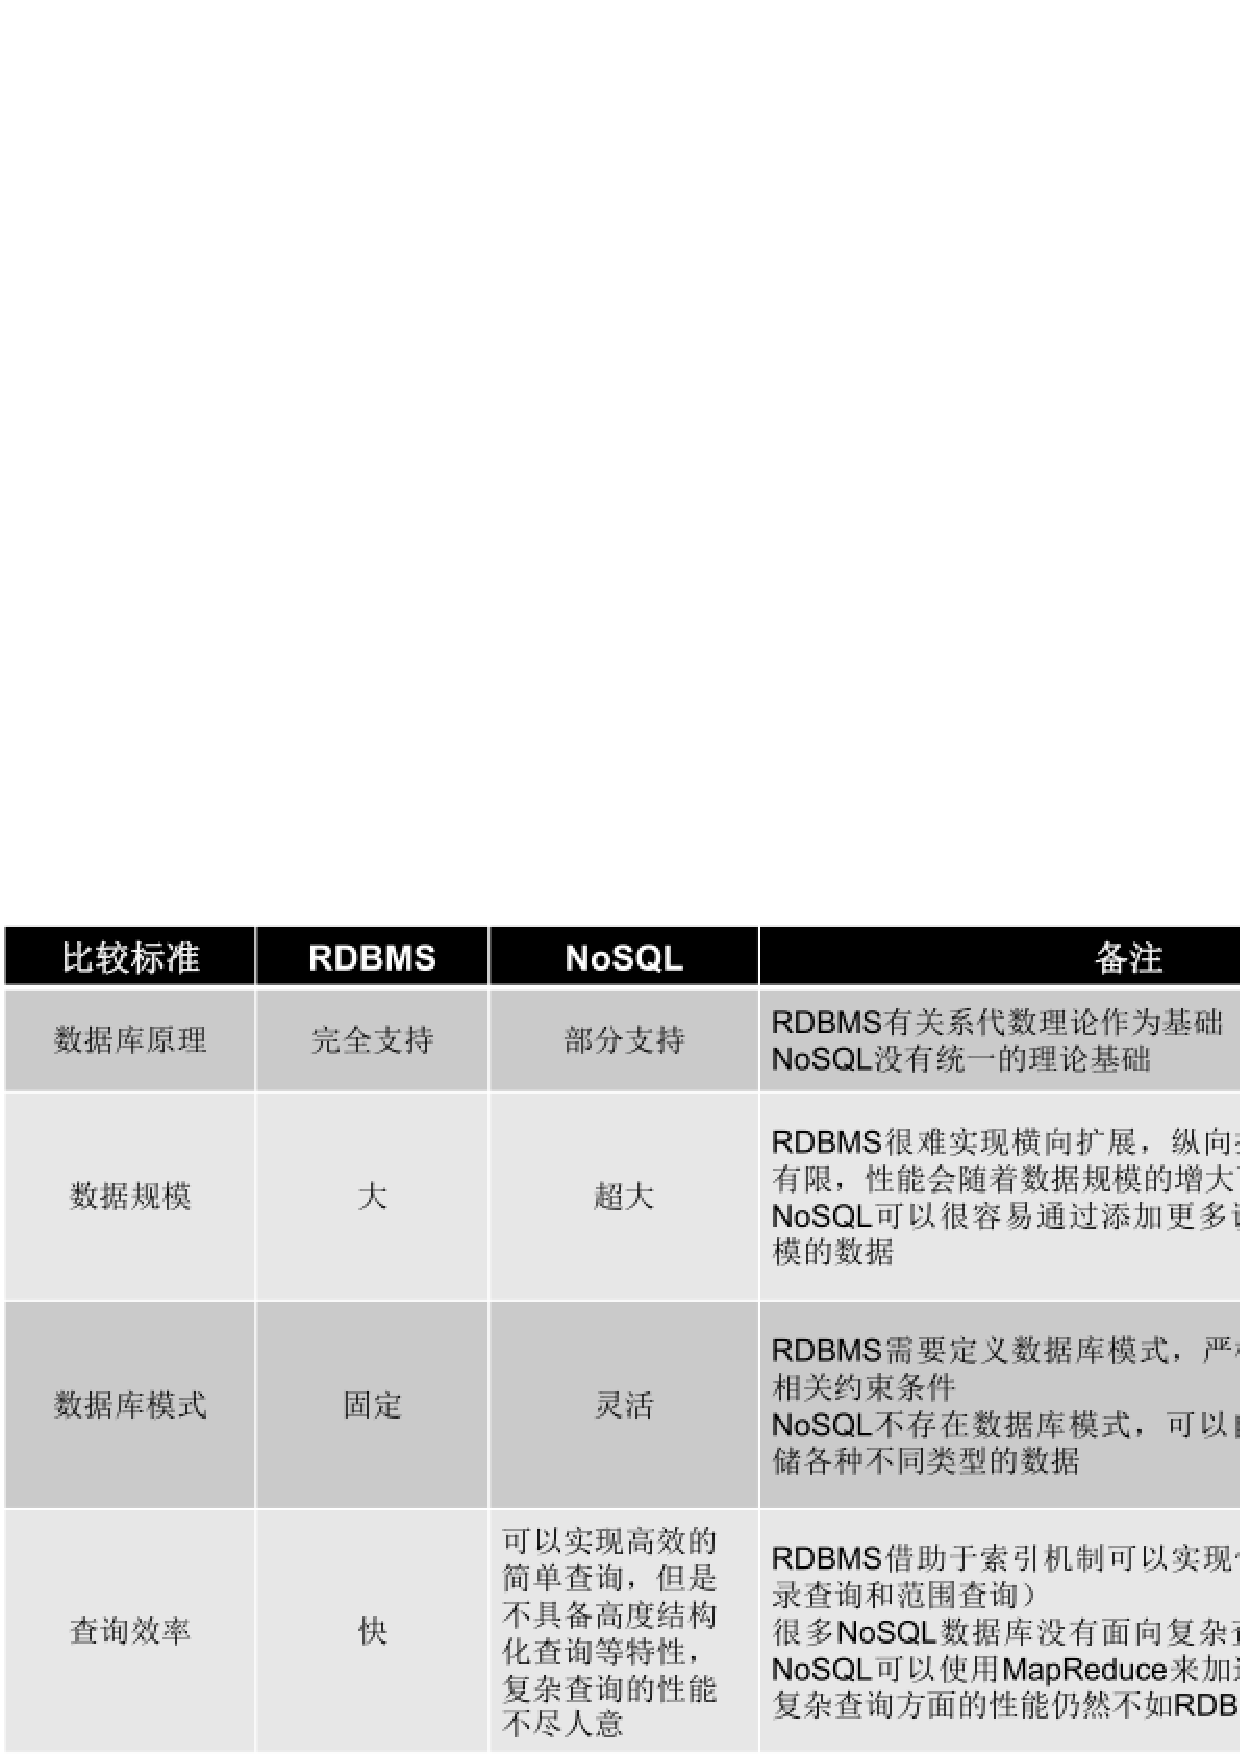
\includegraphics{0.PNG}
    \caption{监督学习的工作方式}
  \end{figure}
  \indent 学习算法学完训练数据后,输出h,h表示一个函数,输入房子的大小x,输出房子的价格y。即:h是x到y的函数映射。h的表达方式有可能是$h_\theta(x)=\theta_0+\theta_1x$。因为只含有一个特征/输入变量,因此这样的问题叫做单变量线性回归问题。

  \section{代价函数}
  代价函数的作用是为我们的模型选择合适的参数$\theta_0$和$\theta_1$。参数决定了我们得到的直线相对于我们的训练集的准确程度,模型所预测的值与训练集中实际值之间的差距就是\textbf{建模误差}。最终目标是选择出可以让\textbf{建模误差的平方和}能够最小的模型参数。即:使代价函数$J(\theta_0, \theta_1)=\frac{1}{2m}\sum_{i=1}^{m}(h_\theta(x^{(i)}-y^{(i)}))^2$最小。

  \begin{figure}[h]
    \centering
    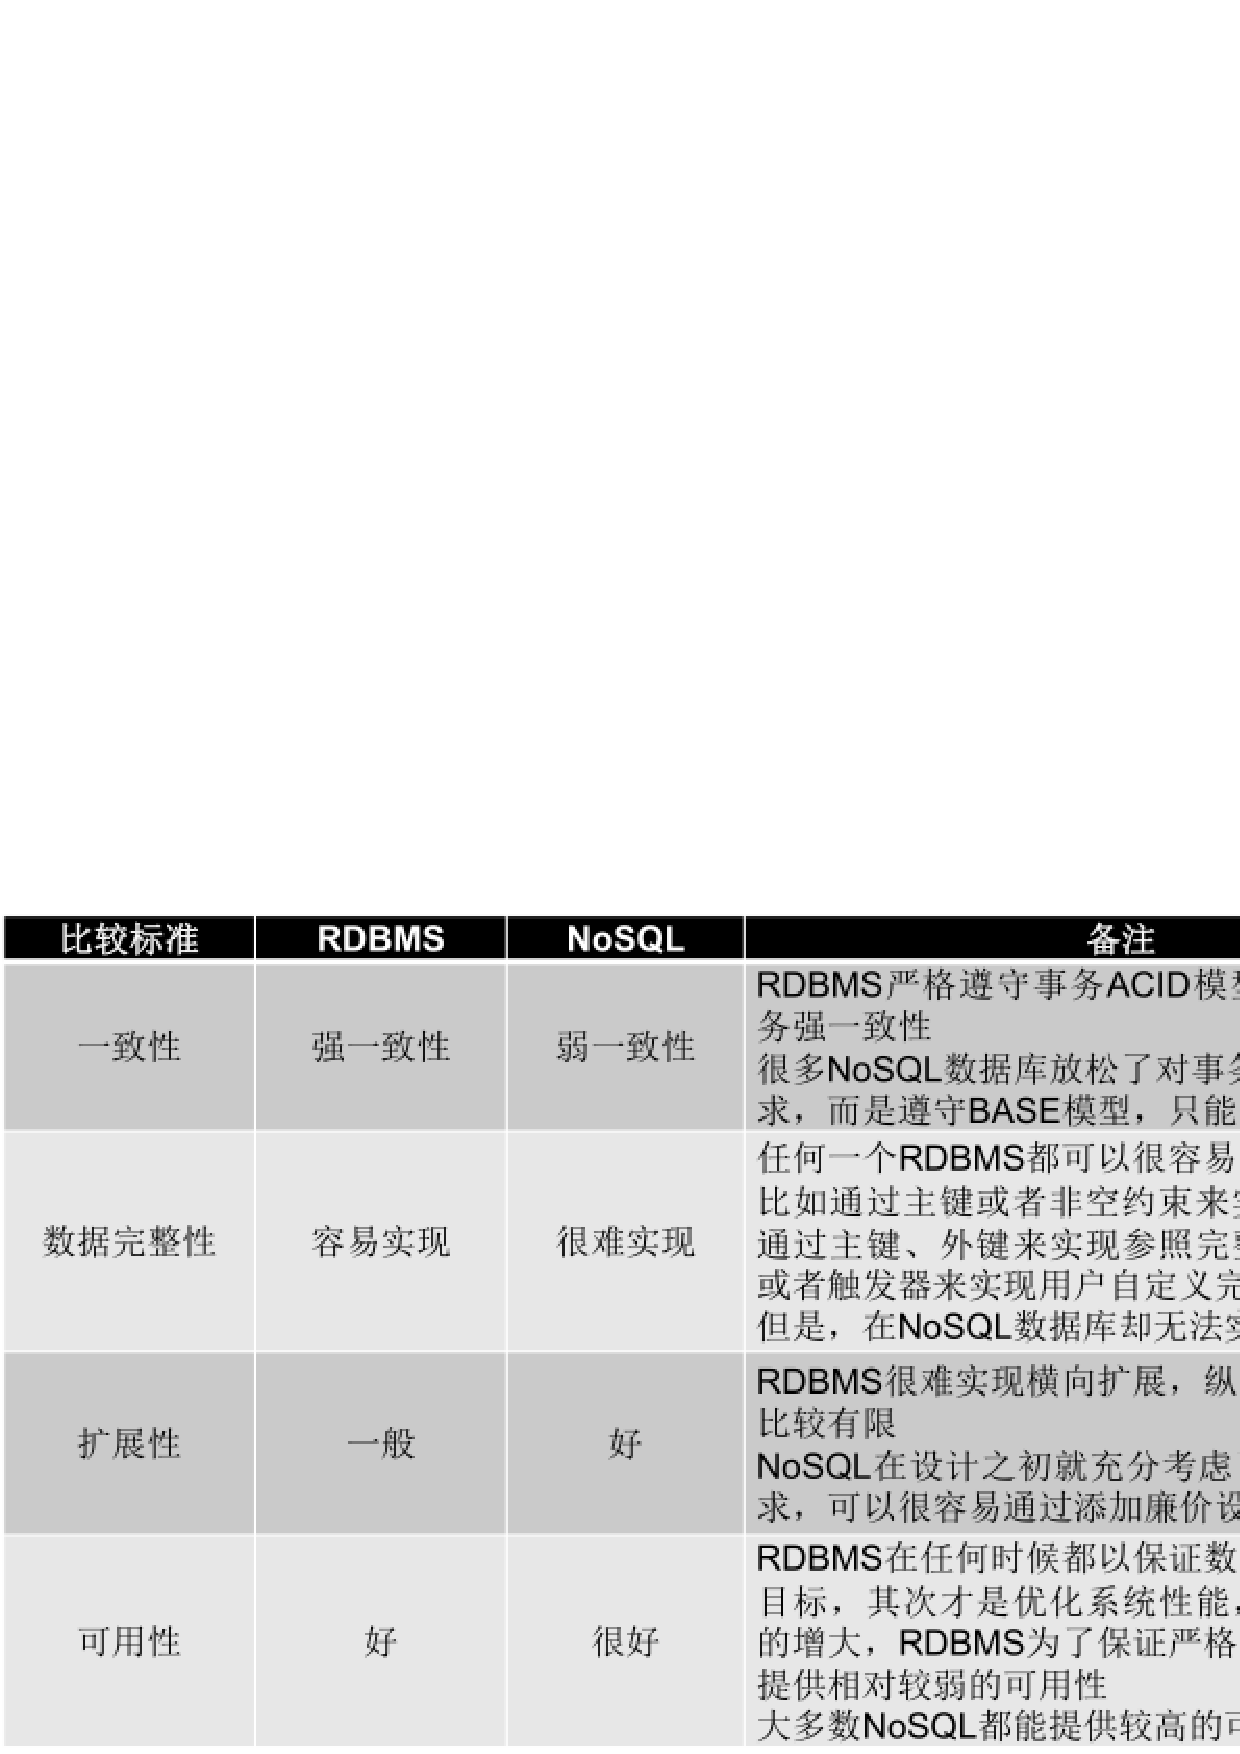
\includegraphics{1.PNG}
    \caption{等高线图}
  \end{figure}
  可以看出,在三维空间中,存在一个使$J(\theta_0, \theta_1)$最小的点。代价函数也称为平方误差函数,之所以选择平方误差函数,是因为对于大部分问题,特别是回归问题,都是一个合理的选择。
\end{large}
\end{document}

%%% Local Variables:
%%% mode: latex
%%% TeX-master: t
%%% End:
